% !TeX root = ../../../main.tex

After the qualitative discussion of the previous sections, here we
present results for the $\cos\theta^*$
distributions Eq.~(\ref{eq:dsigma-dcos}) and the
forward-backward asymmetry Eq.~(\ref{eq:forward-backward-asymmetry}), with
NLO QCD and electroweak corrections included and
with realistic selection and acceptance cuts for the LHC at $\sqrt{s} = 14$~TeV
and different values of the invariant mass $\mll$ relevant for SM
studies and BSM searches.

Computations are performed using {\sc\small MadGraph5\_aMC@NLO}~\cite{Alwall:2014hca},
interfaced to {\sc\small PineAPPL}~\cite{Carrazza:2020gss,christopher_schwan_2022_7023438} to generate
fast interpolation grids.
%
In order to account for realistic detector acceptances,
we impose phase-space cuts on the transverse momentum and the pseudo-rapidity of the two
leading leptons,
\be
p_T^{\ell} > 10~{\rm GeV}  \, ,\qquad |\eta_{\ell}| < 2.4 \,.
\ee
We then consider various regions of dilepton invariant mass $\mll$:
either close to the $Z$-boson peak ($60$~GeV $< \mll < 120$~GeV),
relevant for precision SM studies, or the
high-mass region relevant for BSM searches, with  various choices of a
lower mass invariant cutoff ($\mll > 3,4,5,6$~TeV).
%
In all cases, in order to facilitate the interpretation of
hadron-level results  and the connection to
the discussion of the PDF features from Sect.~\ref{sec:largexpdfs},
we also provide results for the two partonic channels that give the
largest contribution to the cross-section.
%
As in Sect.~\ref{sec:largexpdfs}, we compare results obtained using
the  ABMP16, CT18, MSHT20, and \nnpdfr{4.0} PDF sets.
%
In all cases, we
use the  NNLO sets corresponding to the value $\alpha_s(m_Z)=0.118$
of the strong coupling.
%
Results obtained using the NNPDF3.1 PDF set are reported in App.~\ref{app:nnpdf31}.

%-------------------------------------------------------------------------------
\begin{figure}[!t]
 \centering
 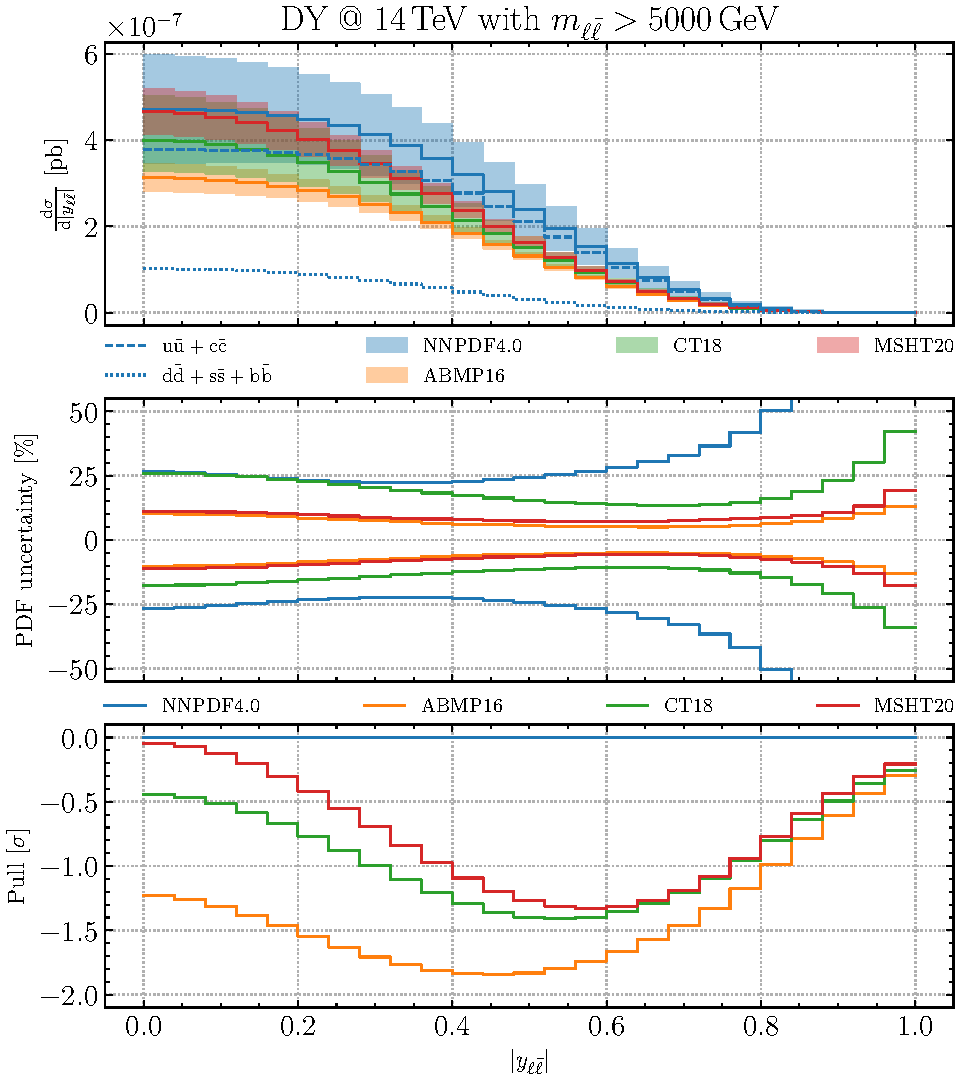
\includegraphics[width=0.49\linewidth]{plots/NNPDF_DY_14TEV_BSM_AFB_YLL_5000}
 \caption{The differential distribution in absolute dilepton rapidity $|\yll|$, given in
Eqn.~(\ref{eq:dsigma-dyll}),
for dilepton invariant masses of $\mll > 5$~TeV
for neutral current Drell-Yan production at the
LHC 14 TeV,
obtained using ABMP16, CT18, MSHT20, and \nnpdfr{4.0} NNLO PDFs with $\alpha_s(m_Z)=0.118$.
%
All
uncertainties shown are 68\% CL PDF uncertainties, computed at NLO
in the QCD and EW couplings with realistic cuts (see text).
We show the absolute distributions (top), relative uncertainties (normalized
to the central curve of each set, middle) and the pull with respect to the
\nnpdfr{4.0} result, Eq.~(\ref{eq:pulldef_xsec}) (bottom).
%
For the central \nnpdfr{4.0} prediction
the contributions of the $u\bar{u}+c\bar{c}$ and $d\bar{d}+s\bar{s}+b\bar{b}$
parton subchannels are also shown.
 \label{fig:CMS_DY_14TEV_MLL_5000_rap}}
\end{figure}
%-------------------------------------------------------------------------------

Before considering the angular distributions, in
Fig.~\ref{fig:CMS_DY_14TEV_MLL_5000_rap} we display the 
differential distribution in absolute dilepton rapidity $|\yll|$,
defined in Eqn.~(\ref{eq:dsigma-dyll}),
for a dilepton invariant mass of $\mll > 5$~TeV.
%
This is the kinematic region relevant for searches of high-mass resonances
in the dilepton channel at the LHC, e.g.~\cite{ATLAS:2019erb,Khachatryan:2016zqb}.
%
We display the absolute differential distributions with the 68\% CL PDF uncertainties
(top), the relative PDF uncertainty (center) normalized for each PDF
set to the corresponding central prediction, and the pull between the
\nnpdfr{4.0} result, taken as a reference, and other sets (bottom).
%
This pull is    defined as
    \be
\label{eq:pulldef_xsec}
{\rm Pull}_i= \frac{ \sigma^{(0)}_{2,i} -\sigma^{(0)}_{1,i} }{
  \sqrt{ \lp  \delta \sigma_{2,i}\rp^2+\lp  \delta \sigma_{1,i}\rp^2 }} \, , \qquad i=1,\ldots,n_{\rm bin} \, ,
\ee
where  $\sigma^{(0)}_{1,i}$ and $\sigma^{(0)}_{2,i}$ are the central values of the
theory prediction in the $i$-th bin of the distribution and $\delta \sigma_{1,i}$, $\delta \sigma_{2,i}$ are
the corresponding PDF uncertainties.
%
For the central \nnpdfr{4.0} prediction in the upper panel we also display the
contributions from the dominant parton subchannels, namely
$u\bar{u}+c\bar{c}$ and $d\bar{d}+s\bar{s}+b\bar{b}$.

As discussed in Sect.~\ref{sec:HMDY}, the  $|y_{\ell\bar{\ell}}|$  distribution
depends  on the symmetric partonic luminosities $\mathcal{L}_{S,q}$, Eq.~(\ref{eq:lumiss_qpm}),
which in turn are driven by the total PDFs $xf^+_q$.
%
The $|y_{\ell\bar{\ell}}|$  distribution
is dominated by the $u\bar{u}$
contribution and its qualitative behaviour is found to be similar for the four PDF sets considered.
%
PDF uncertainties are the largest in \nnpdfr{4.0}, ranging between 25\% and 50\%,
and the pull between \nnpdfr{4.0} and  CT18 and MSHT20 is at most at the
$1.5\sigma$ level, and slightly larger  
with ABMP16.
%
The dependence of the $|y_{\ell\bar{\ell}}|$  distribution on the dilepton mass $\mll$
is moderate, and the same qualitative features are
obtained if $\mll$ is lowered down to the $Z$-peak region, or
raised to yet higher values.
%
Hence, for the absolute rapidity distribution there is a
reasonable agreement between all  PDF sets for all scales considered.

%-------------------------------------------------------------------------------------
\begin{figure}[t]
\centering
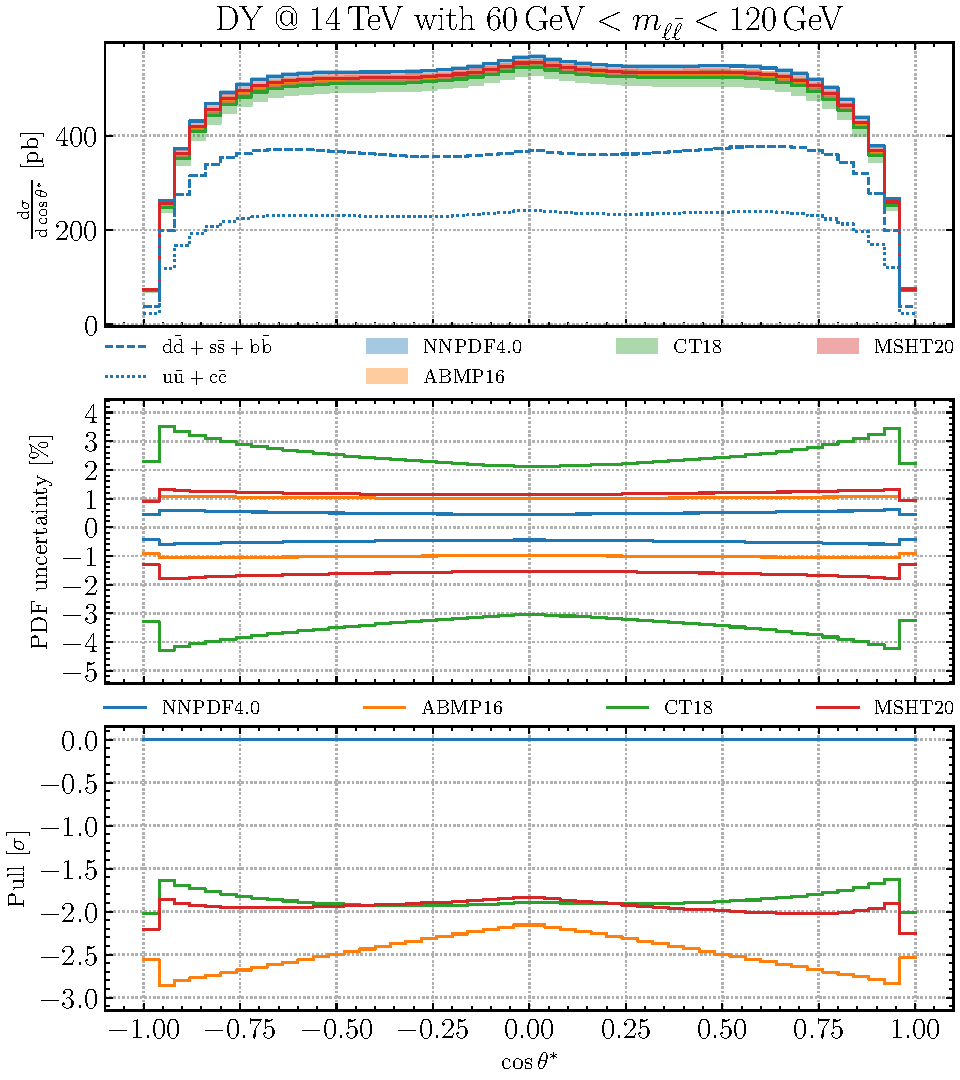
\includegraphics[width=0.49\linewidth]{plots/NNPDF_DY_14TEV_BSM_AFB_COS_060_120}
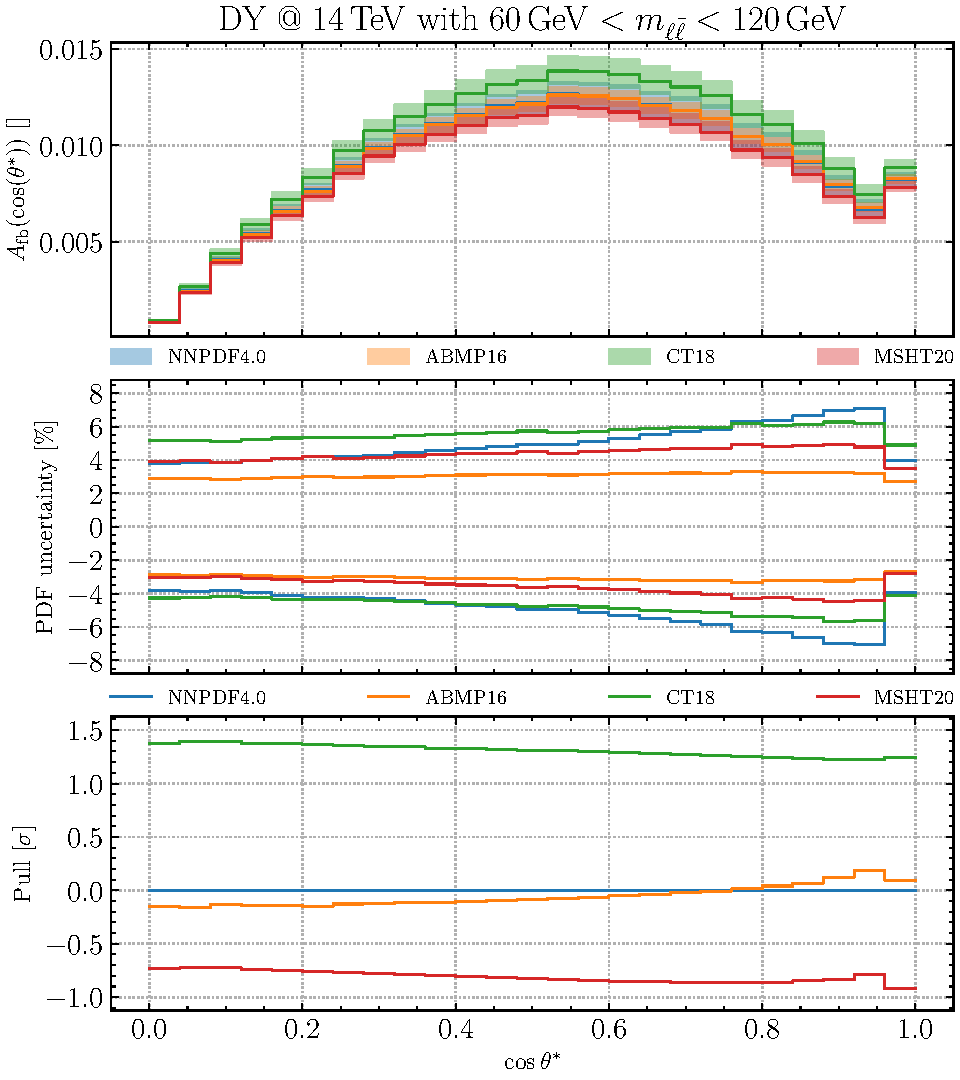
\includegraphics[width=0.49\linewidth]{plots/NNPDF_DY_14TEV_BSM_AFB_COS_060_120-afb}
\caption{Same as Fig.~\ref{fig:CMS_DY_14TEV_MLL_5000_rap}, now for the differential distribution in
  $\cos\theta^*$ (left)
  and the corresponding forward-backward asymmetry
  $A_{\rm fb}(\cos\theta^*)$ (right), in the $Z$-peak region defined by $60~{\rm GeV} < \mll < 120$ GeV.}
\label{fig:CMS_DY_14TEV_MLL_zpeak}
\end{figure}
%-------------------------------------------------------------------------------------

We now turn to the differential distribution in
  $\cos\theta^*$ 
  and the corresponding forward-backward asymmetry $A_{\rm
    fb}(\cos\theta^*)$.
We first consider the $Z$-peak region, $60~{\rm GeV} < \mll <
120$~GeV, in Fig.~\ref{fig:CMS_DY_14TEV_MLL_zpeak}.
%
The $\cos\theta^*$ 
distribution exhibits a small but non-negligible asymmetry,
and uncertainties are  smallest for \nnpdfr{4.0}.
%
The four PDF sets predict a similar behaviour and magnitude
of the asymmetry $A_\mathrm{fb}$.
%
PDF uncertainties in the asymmetry
are  comparable for  all PDF sets when $\cos\theta^* \approx0$,
and actually  largest for \nnpdfr{4.0} when $\cos\theta^* \approx 1$.
In all cases the predictions are compatible within $2 \sigma$,
with ABMP16 showing larger differences of up to $2.8 \sigma$ for the $\cos\theta^*$
distribution.
%
Note that the
sharp drop-off at the edges $|\cos\theta^*| \approx  1$, appearing in
all plots in this section, is a consequence of the phase-space cuts which
limit the phase-space volume.
%
Indeed, using  LO kinematics
\begin{equation}
| \cos\theta^* | = \tanh \left| \frac{\eta_\ell - \eta_{\bar{\ell}}}{2} \right| = \sqrt{1 - \frac{4 (p_T^\ell)^2}{\mll^2}} \text{,}
\end{equation}
so $| \cos\theta^* | \approx 1$ requires a lepton pair with either
a large rapidity separation, or a very large invariant mass and small
transverse momenta. 

As expected from the antisymmetric partonic luminosities studied in
Sect.~\ref{subsec:partoniclumis}, the situation is quite different when
considering distributions with a higher dilepton invariant mass range.
%
The angular distribution and forward-backward asymmetry
in the high-mass region, for different values of the  lower cut in the dilepton
 invariant mass, namely $\mll^{\rm min}=3, 4,5$ and 6 TeV, are
 respectively
 shown in
Fig.~\ref{fig:CMS_DY_14TEV_MLL_others} and Fig.~\ref{fig:CMS_DY_14TEV_MLL_others_asy}.

%-------------------------------------------------------------------------------
\begin{figure}[t!]
 \centering
 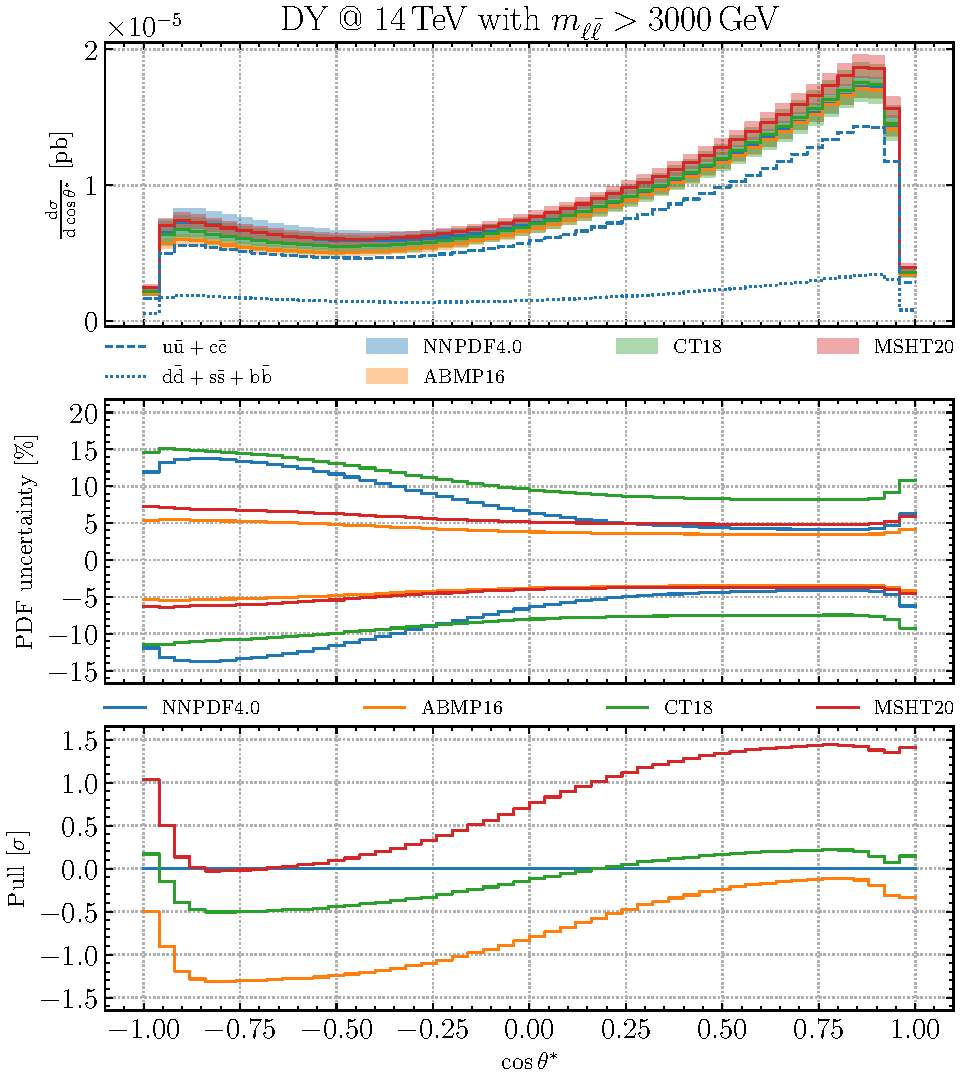
\includegraphics[width=0.49\linewidth]{plots/NNPDF_DY_14TEV_BSM_AFB_COS_3000}
 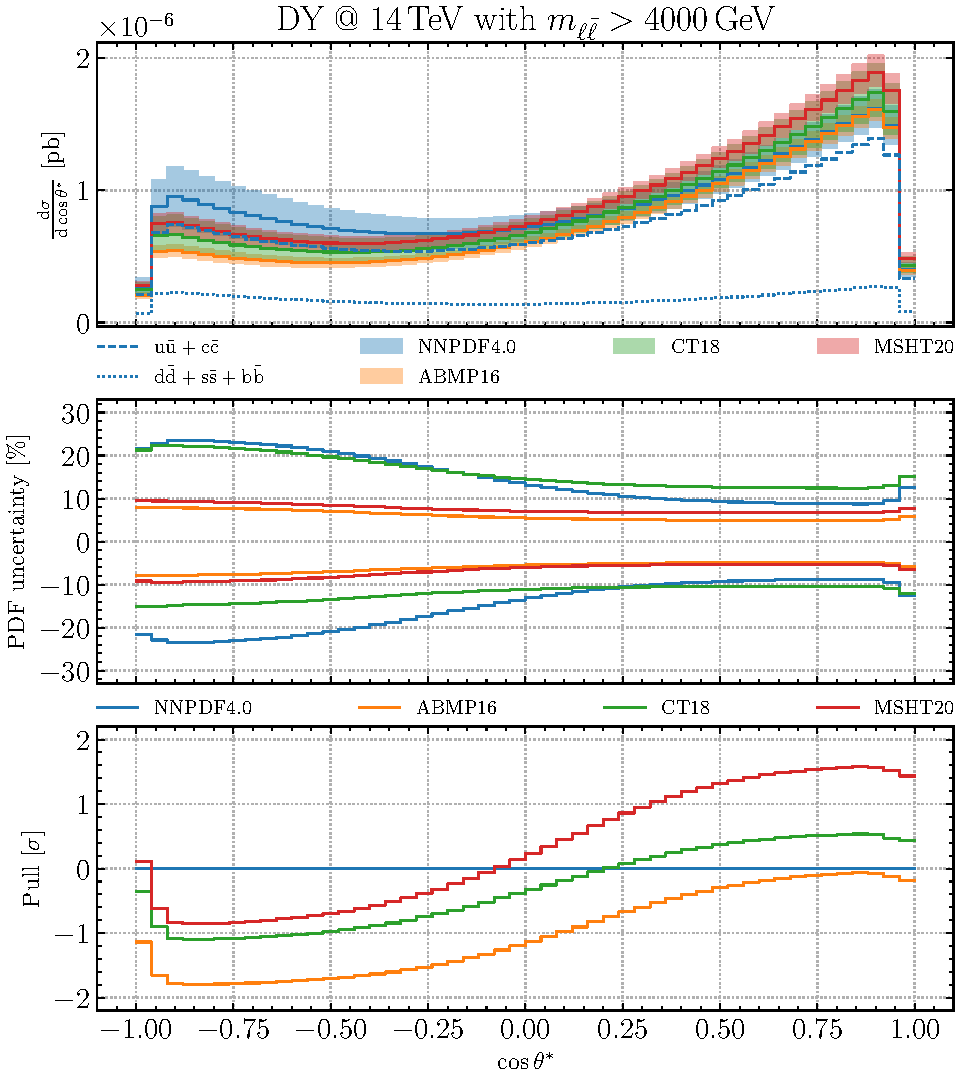
\includegraphics[width=0.49\linewidth]{plots/NNPDF_DY_14TEV_BSM_AFB_COS_4000}
 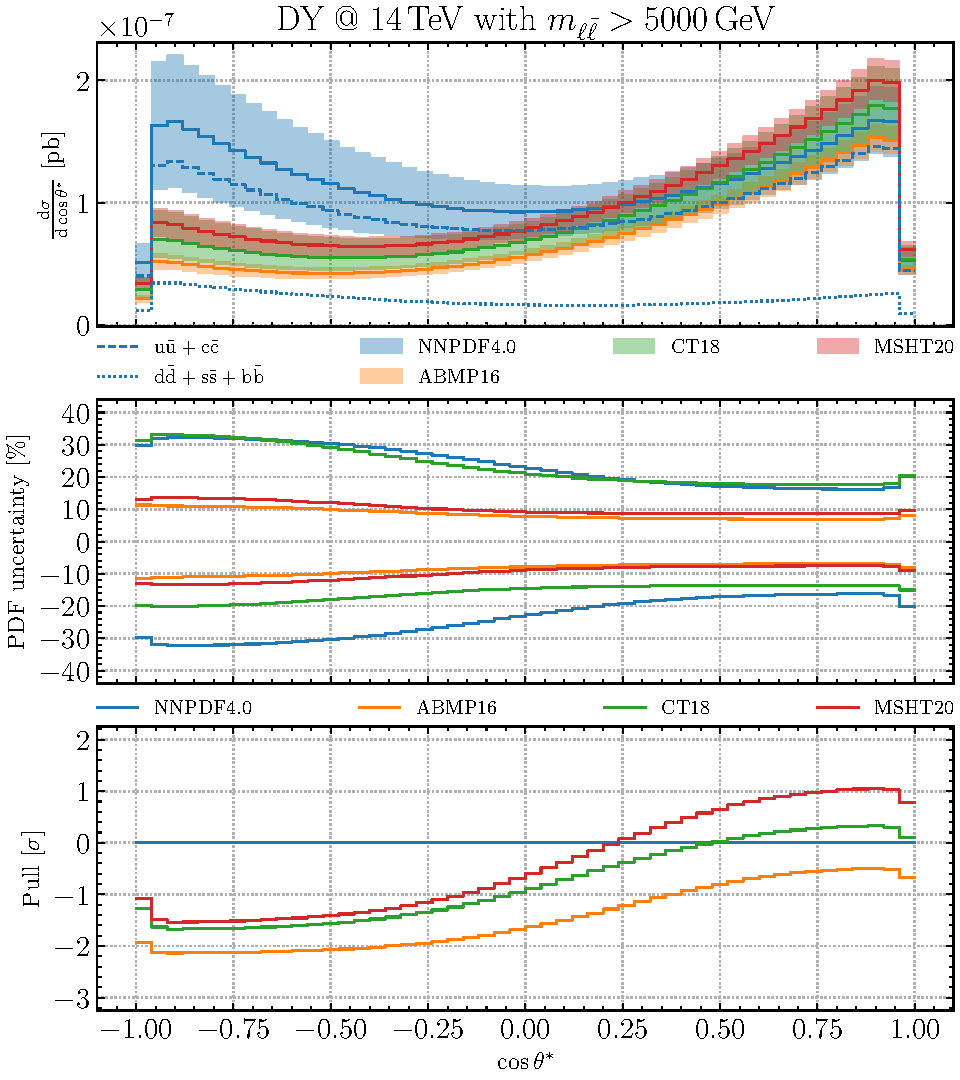
\includegraphics[width=0.49\linewidth]{plots/NNPDF_DY_14TEV_BSM_AFB_COS_5000}
 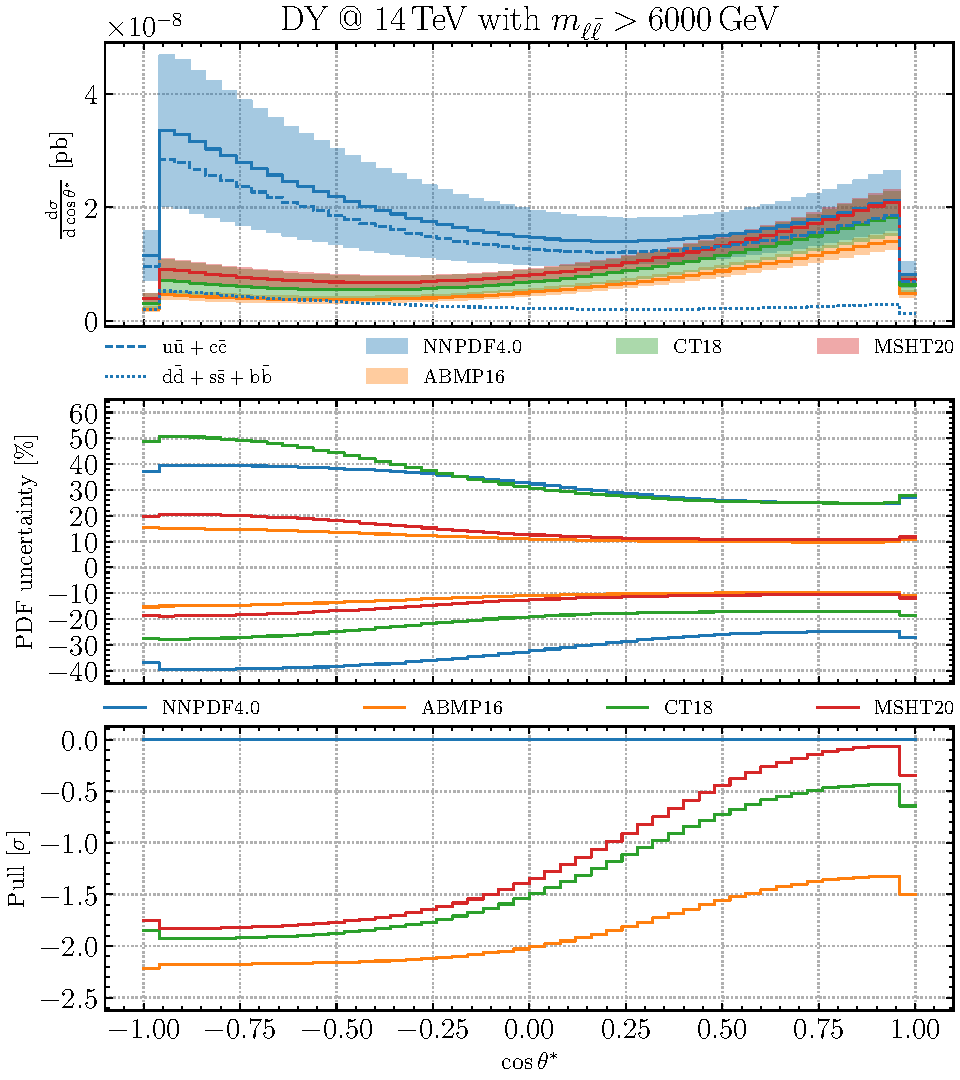
\includegraphics[width=0.49\linewidth]{plots/NNPDF_DY_14TEV_BSM_AFB_COS_6000}
 \caption{Same as Fig.~\ref{fig:CMS_DY_14TEV_MLL_zpeak} (left)
   for different values of the  lower cut in the dilepton
   invariant mass: $\mll \ge 3, 4,5,$ and 6 TeV respectively.
  }    
 \label{fig:CMS_DY_14TEV_MLL_others}
\end{figure}
%-------------------------------------------------------------------------------

 Consistent with the underlying parton luminosities, the $\cos\theta^*$ distribution
 is dominated by $u\bar{u}$ scattering, while  $d\bar{d}$ provides
 a subdominant contribution.
 %
 When the lower cut  is $\mll^{(\rm min)}=3$ TeV is used, the four PDF
 sets are in agreement at the $1\sigma$ level: they all
 display a 
 positive forward-backward asymmetry, and exhibit PDF uncertainties ranging between 10\% and 15\%.
 %
 As the invariant mass cut is raised, the qualitative behaviour of the
 angular distribution and
 asymmetry change substantially for \nnpdfr{4.0}, while they remain
 approximately the same for all other PDF sets, consistent with the
 behaviour of the PDFs and luminosities discussed in
 Sect.~\ref{sec:subsec-largexPDFs}-\ref{subsec:partoniclumis}.
%
 Specifically,
 raising the cut to
 $\mll \ge 4$ TeV, for \nnpdfr{4.0}
 the backwards cross-section starts increasing, though the asymmetry remains
positive.
 %

For $\mll\ge 5$ TeV the central value of the \nnpdfr{4.0} $\cos\theta^*$
 distribution  becomes symmetric, though the  PDF uncertainty band is
 rather asymmetric. Also, PDF uncertainties
 are now the largest for \nnpdfr{4.0}, reaching up to 30\%.
 %
 Finally, for $\mll\ge 6$ TeV  the central value of 
 forward-backward asymmetry for \nnpdfr{4.0} becomes negative, with the
 PDF uncertainties increasing further so the asymmetry remains compatible
 with zero at about the 1.1~$\sigma$ level.
   %
 For all other PDF sets there is little change in the shape of the distribution as the
 dilepton invariant mass cut is increased.

%-------------------------------------------------------------------------------
\begin{figure}[t!]
 \centering
 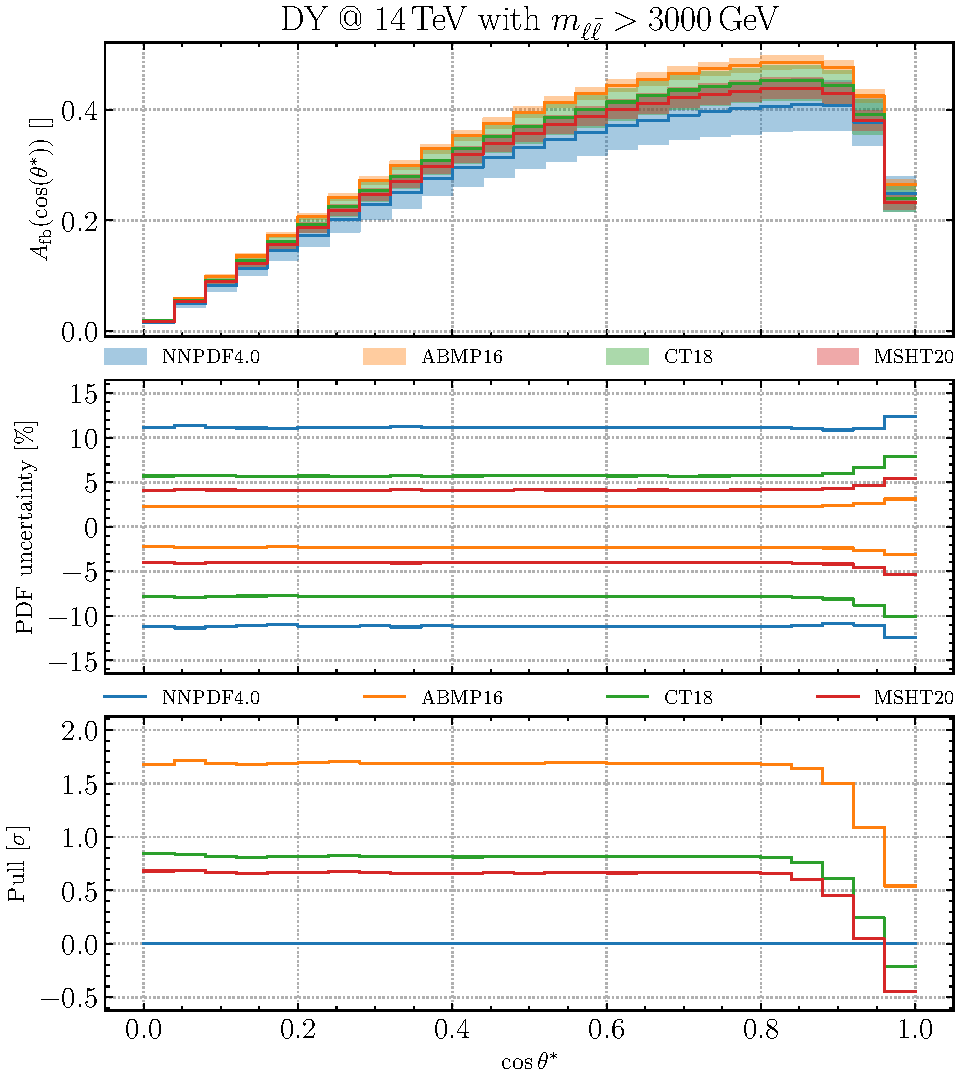
\includegraphics[width=0.49\linewidth]{plots/NNPDF_DY_14TEV_BSM_AFB_COS_3000-afb}
 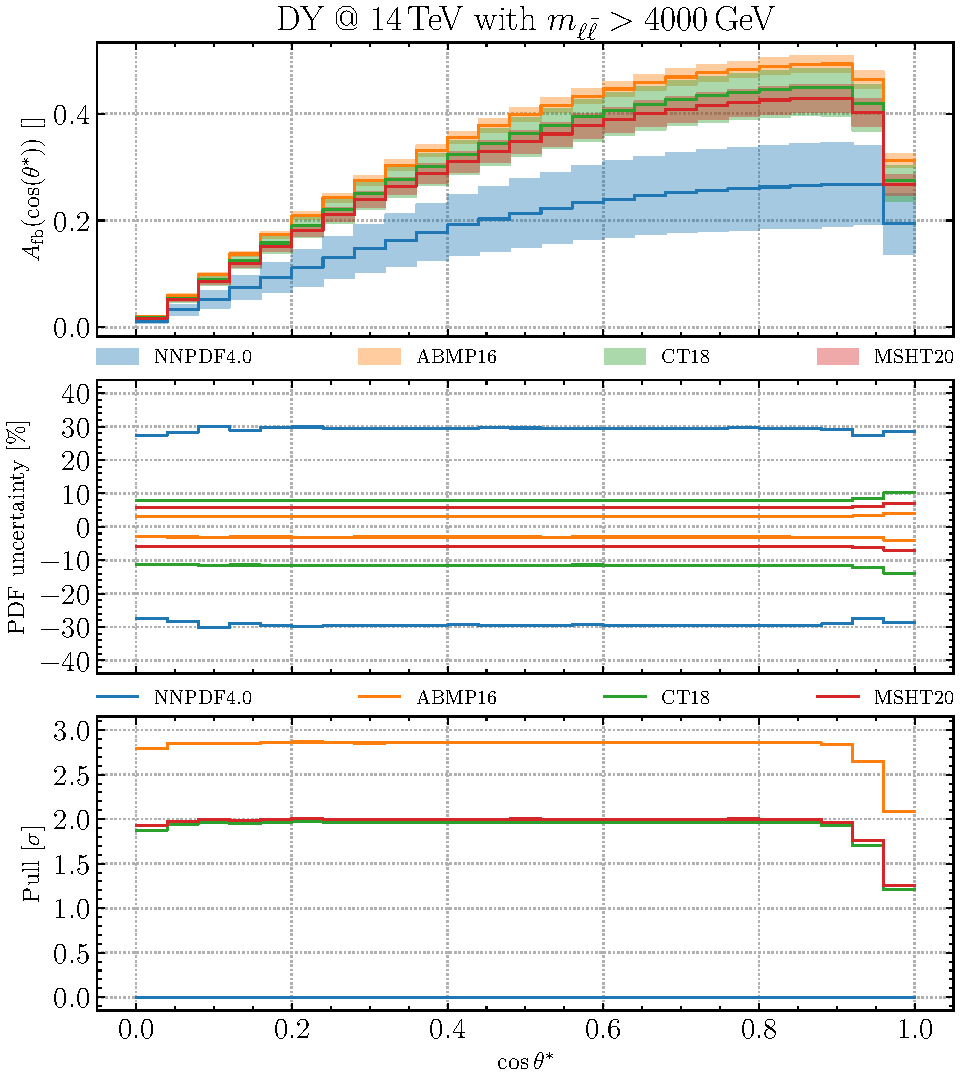
\includegraphics[width=0.49\linewidth]{plots/NNPDF_DY_14TEV_BSM_AFB_COS_4000-afb}
 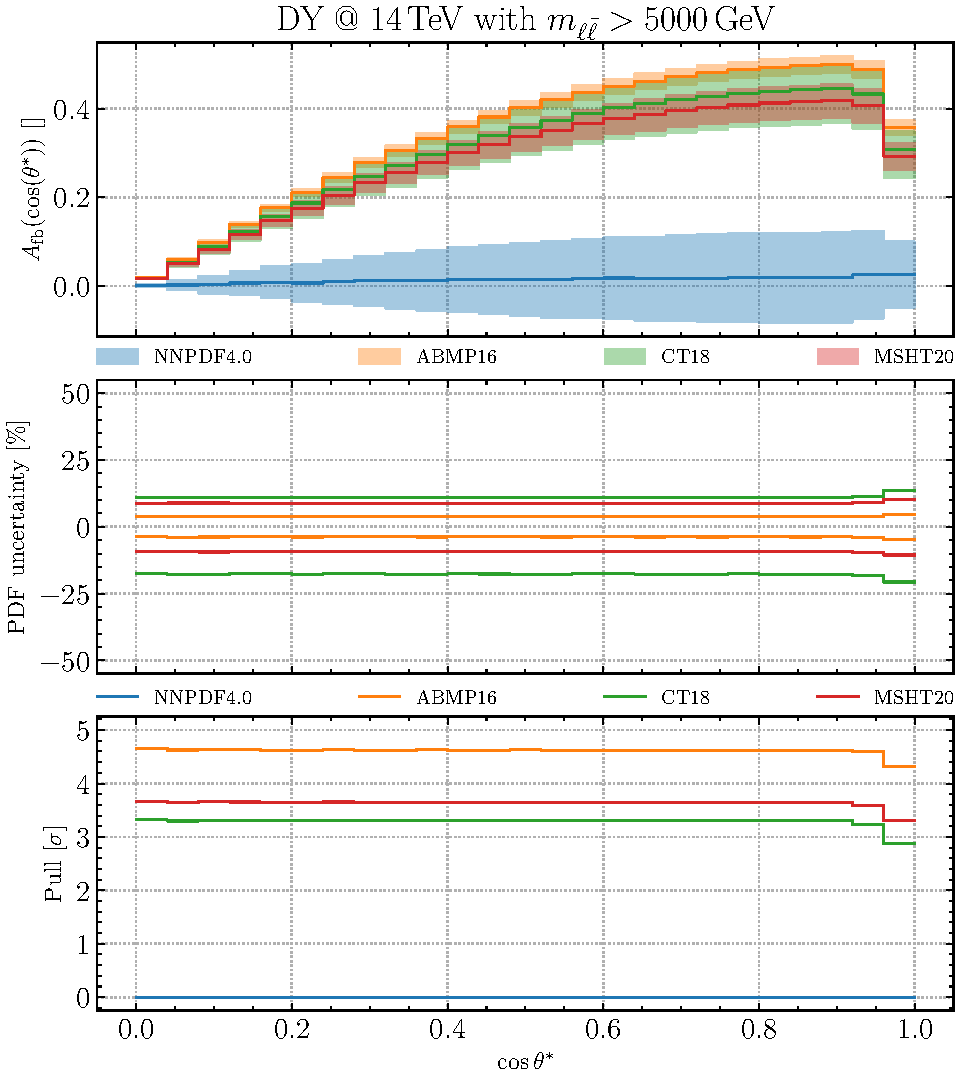
\includegraphics[width=0.49\linewidth]{plots/NNPDF_DY_14TEV_BSM_AFB_COS_5000-afb}
 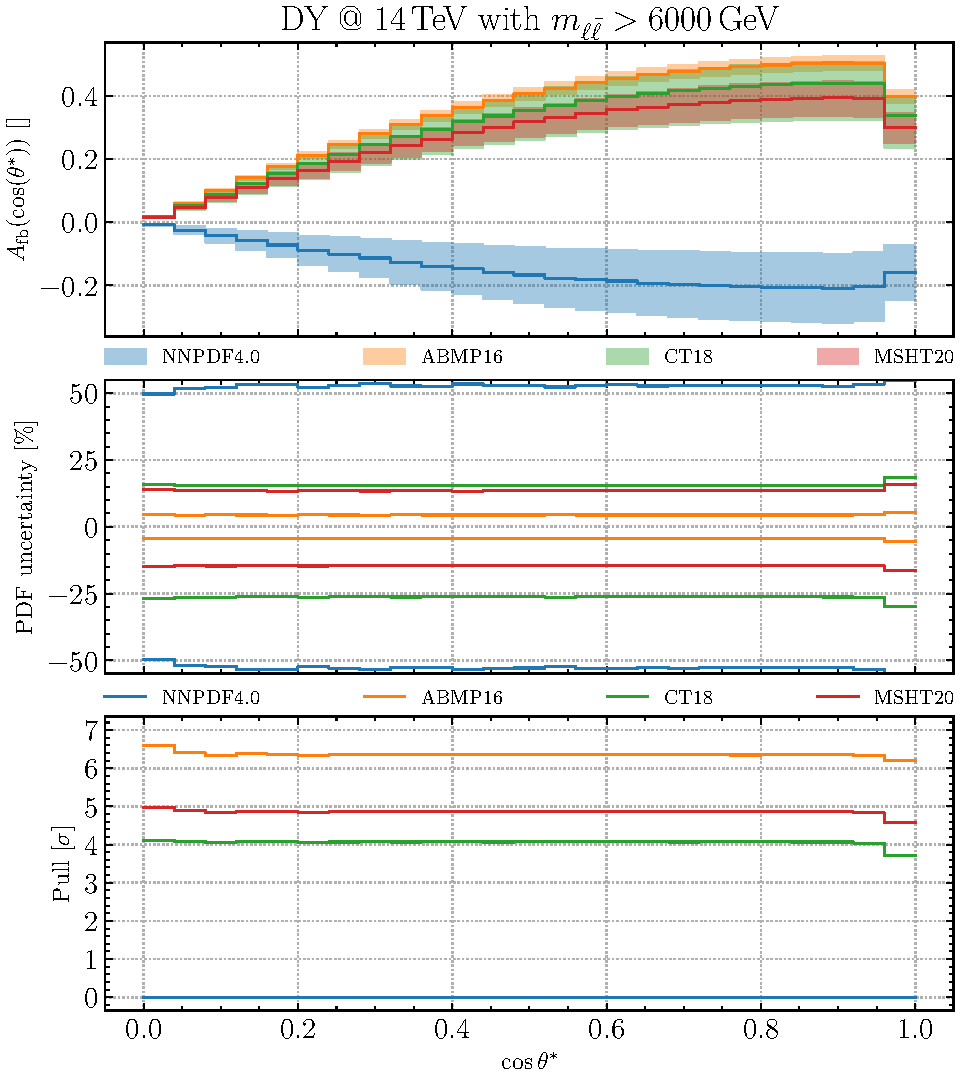
\includegraphics[width=0.49\linewidth]{plots/NNPDF_DY_14TEV_BSM_AFB_COS_6000-afb}
 \caption{Same as Fig.~\ref{fig:CMS_DY_14TEV_MLL_zpeak} (right)
   for different values of the  lower cut in the dilepton
   invariant mass: $\mll^{\rm min}=3, 4,5,$ and 6 TeV.
  }    
 \label{fig:CMS_DY_14TEV_MLL_others_asy}
\end{figure}
%-------------------------------------------------------------------------------

Because of the very large uncertainty on the \nnpdfr{4.0} result for the $\cos\theta^*$
distribution, even with
the highest value of the  $\mll^{(\rm  min)}$ cut, where \nnpdfr{4.0} finds a
symmetric distributions while all other PDF sets find an asymmetry,
the pull is always below $2 \sigma$.
%
This suggests that the more
conservative estimate of  \nnpdfr{4.0} in the extrapolation region might be
desirable, and lead to more robust predictions for the
forward-backward asymmetry in the high-mass region which is relevant
for new physics searches.
